\section{Territory}
\begin{itemize}
    \item Territory is an essential element of statehood; it is within territory that a state's legal authority is exercised
    \item Sovereignty in relation to territory is ``the right to exercise therein, to the exclusion of any other State, the functions of a State'' -- \case{\textit{Island of Palmas} (1928)} (Judge Huber)
    \item States generally have complete authority over what happens within their territory, subject to international law
    \item ``The basic legal concept of State sovereignty in customary international law, expressed in ... Art 2(1), of the UN Charter, extends to the internal waters and territorial sea of every State and to the air space above its territory'' -- \case{\textit{Nicaragua} [1986] ICJ Rep 14}
    \item There is a distinction between sovereignty (dominium) and jurisdiction (imperium)
    \begin{itemize}
        \item For example, there are some areas (e.g., maritime areas) where states do not have sovereignty/ownership, but enjoy extensive jurisdictional rights (e.g., an exclusive economic zone (EEZ), where they have jurisdiction to regulate access to the zone, and access to the resources within it, but they do not have sovereignty over it)
        \item It is only in some circumstances where jurisdiction can extend beyond areas of sovereignty
    \end{itemize}
\end{itemize}

\section{Modes of Acquiring Territory}
\subsection{Occupation}
\begin{itemize}
    \item Occupation is the formal act of intention and demonstration of effective control over territory
    \item The territory must be unoccupied (i.e., not subject to the sovereignty of another state)
    \item Territory may be acquired through occupation if it is \textit{terra nullius} (i.e., no population, or if the territory is abandoned)
    \item This generally occurs through physical settlement, but only when the territory is uninhabited or abandoned (at which points it is considered \textit{terra nullius})
    \item Occupation is ``an original means of peaceably acquiring sovereignty over territory'' -- \case{\textit{Western Sahara Advisory Opinion} [1975] ICJ Rep 162}
\end{itemize}

\begin{casedetails}{\textit{Western Sahara Advisory Opinion} [1975] ICJ Rep 162}
    \flushleft
    This case concerned a dispute over sovereignty to West Sahara, which was formerly a Spanish colony. It was claimed by both Morocco (on the basis of Spain's former colonisation), and by Mauritania. The ICJ was asked by the UNGA about the status of Western Sahara. It held that occupation was only valid if it was \textit{terra nullius}.

    \vspace{\baselineskip}

    In its Advisory Opinion, the ICJ noted at [80] that ``territories inhabited by tribes or peoples having a social and political organization [are] not regarded as terrae nullius''. Moreover, colonial occupation was often not of \textit{terra nullius}, but through agreement with local rulers. Western Sahara was inhabited by nomadic peoples, who were nonetheless socially and politically organised. Moreover, there were no ties to Morocco or Mauritania so as would disrupt or upset decolonisation and self-determination.

    \vspace{\baselineskip}

    \textbf{From this case, it is held that there can only be a valid occupation if the territory is truly \textit{terra nullius}.} In this instance, it was an enormous territory inhabited by relatively few people, but the ICJ held that this was not necessarily problematic, nor that the peoples occupying in Western Sahara were nomadic. The tribes in Western Sahara were socially and politically organised, and did effectively occupy the territory. The ICJ also held that when Spain colonised Western Sahara, it did not argue that it was occupying Western Sahara. The Spanish King in 1884 instead stated that he was taking the area of Western Sahara under his protection on the basis of agreements entered into with local rulers, which does not indicate an occupation.

    \vspace{\baselineskip}

    The process of self-determination remains incomplete (Western Sahara is often considered Africa's last colony), with completing claims by the Sahrawi Arab Democratic Republic (Polisario), and Morocco.
\end{casedetails}

\begin{casedetails}{\textit{Mabo v Queensland (No 2)} (1992) 175 CLR 1}
    \flushleft
    The question arising from this case was that when the British invaded Australia, did they acquire sovereignty over the land, but also acquire land rights that had the effect of extinguishing any pre-existing land rights held by the Indigenous occupants of Australia?

    \begin{longtable}{p{0.1\textwidth}|>{\raggedright\arraybackslash}p{0.85\textwidth}}
        Brennan J at [41] & If the international law notion that inhabited land may be classified as terra nullius no longer commands general support, the doctrines of the common law which depend on the notion that native peoples may be "so low in the scale of social organization" that it is ``idle to impute to such people some shadow of the rights known to our law" (In re Southern Rhodesia (1919) AC, at pp 233-234) can hardly be retained. If it were permissible in past centuries to keep the common law in step with international law, it is imperative in today's world that the common law should neither be nor be seen to be frozen in an age of racial discrimination. \\\hline
        Brennan J at [47] & The acquisition of territory is chiefly the province of international law; the acquisition of property is chiefly the province of the common law. \\\hline
        Deane and Gaudron JJ at [3] & [T]here are problems about the establishment of the Colony in so far as the international law of the time is concerned… contemporary international law would seem to have required a degree of actual occupation of a "discovered" territory over which sovereignty was claimed by settlement and it is scarcely arguable that the establishment by Phillip in 1788 of the penal camp at Sydney Cove constituted occupation of the vast areas of the hinterland of eastern Australia…However, in so far as the establishment of British sovereignty is concerned, those problems do not exist for the purposes of our domestic law.
    \end{longtable} 

    Brennan J held that international law never regarded territory that was occupied as \textit{terra nullius}. Consequently, the common law must disregard this fiction that Australia was \textit{terra nullius} at the time of British colonisation.

    \vspace{\baselineskip}

    Deane and Gaudron JJ held that whilst the prerogatives of the Crown to acquire territory were in question, from the perspective of domestic law, we cannot question whether the territory was lawfully acquired (as this was a power of the Crown at the time in the eyes of domestic law, and hence could not be questioned). The Court can be look at what happens with the common law, and that the acquisition of radical title over Australia by Britain did not have the effect of extinguishing, in all circumstances, pre-existing native title.
\end{casedetails}

\subsubsection{Intention to Occupy}

\begin{itemize}
    \item For an intention to occupy to be manifest:
    \begin{itemize}
        \item There must be an expression of formal intent to claim possession of the land (e.g., the planting of a flag); this is known as \textit{animus occupandi}
        \item There must be a demonstration of effective control
        \item Territory must be claimed by a state authority, not a private actor
        \begin{itemize}
            \item If a private citizen holds state authority to claim territory, this is generally sufficient, but it needs to be done by a state organ
        \end{itemize}
    \end{itemize}
    \item Under Australian law, individuals may not acquire title in unoccupied land not claimed by a state, following \case{\textit{Ure v Commonwealth} [2016] FCAFC 8} (Page \pageref{case:Ure v Commonwealth})
    \begin{itemize}
        \item Private individuals cannot claim/acquire title in \textit{terra nullius}
    \end{itemize}
\end{itemize}

\subsubsection{Effective Occupation}
\begin{itemize}
    \item For there to be effective occupation, there must be:
    \begin{itemize}
        \item A continuous and peaceful display of state authority
        \item A responsible authority that exercises governmental functions (\textit{effectivités})
        \item Spatial extent (although not necessarily all territory), duration, continuity, and peacefulness are all relevant considerations
    \end{itemize}
    \item It is not normally essential that a state has control over every exact area of land of their territory; this requirement tends to be relaxed especially in relation to remote/hard-to-access areas
\end{itemize}

\begin{casedetails}{\textit{Clipperton Island Arbitration (France v Mexico)} 1932}
    \flushleft
    This case concerned a dispute between France and Mexico over the sovereignty of Clipperton Island, which was 1200km off the coast of Mexico. In 1897, a Mexican naval vessel landed and raised a flag, claiming success to title on the basis of Spanish discovery in 1836. However, Spain did not incorporate the island into its territory. A French naval officer on a private vessel claimed the uninhabited island in 1858 as French territory.

    \vspace{\baselineskip}

    Mexico had not exercised sovereignty over the island before the arrival of the French sailors, and so the land was \textit{territorium nullius}. On the other hand, France had ``made known in clear and precise manner [its] intention to consider [the] island her territory''.
    
    \vspace{\baselineskip}

    It is generally the case that there must also be effective occupation in claiming the land, by establishing within the territory an organisation to give effect to laws (this was not considered here, however, due to the remoteness of the territory).
\end{casedetails}

\subsection{Cession}
\begin{itemize}
    \item Cession is the intentional transfer of sovereignty over territory from one state to another
    \item it is a consensual/voluntary process, and can be done for either a price or for free
\end{itemize}

\subsection{Prescription}
\begin{itemize}
    \item Prescription is the acquisition of title to territory formerly occupied by another state through a peaceful exercise of sovereignty
    \item It bears a number of similarities to a doctrine of Roman law and aspects of common law, and is an idea of `squatter's rights'
    \item In cases of possession, the other state has a valid title to territory, but is not actively asserting their right to that title, and so the possessing state eventually gains title by occupying it; it turns a possessory interest into a fully proprietary interest
    \item Prescription can also be considered as the legitimisation of a doubtful title through the passage of time (e.g., adverse possession and immemorial possession)
    \item There are a number of criteria for prescription:
    \begin{itemize}
        \item \textit{À titre de souverain} (in exercise of sovereign powers)
        \begin{itemize}
            \item The possession has to be under state authority; it cannot be by a private actor
        \end{itemize}
        \item Peaceful possession
        \begin{itemize}
            \item Prescription cannot be claimed when there was a conflict/war; this would instead be considered conquest, which is illegal under international law
        \end{itemize}
        \item Public
        \begin{itemize}
            \item Prescription must be made publicly known
        \end{itemize}
        \item Uninterrupted
        \item Endure for a length of time
        \item Acquiescence by the other state
        \begin{itemize}
            \item This is a contested point
            \item The original title holder must have acquiesced to the acquisition of title by the new owner
            \item The original title holder may (meekly) protest to some extent, or otherwise stop asserting their title, which evinces an intention to surrender their title over the land
        \end{itemize}
    \end{itemize}
\end{itemize}

\begin{casedetails}{\textit{Island of Palmas Case (Netherlands v US)} (1928)}
    \flushleft
    This case concerned a dispute between the Netherlands and the US over the sovereignty of Palmas Island, which was located between the Philippines and Indonesia. The US claimed title to the island on the basis of discovery, but the Netherlands claimed title on the basis of prescription. The Philippines ceded the island to the US after the 1898 Spanish-American war (an example of cession), but in 1906 the US discovered the Dutch flag flying on Palmas (the US thought they had title over the Philippines as it had been given to them by the Spaniards). The Netherlands claimed title n the basis of acts of state authority that they had exercised from 1677 onwards.

    \vspace{\baselineskip}

    Judge Huber held that the island was part of the Netherlands. On the topic of Spain's apparent discovery, he he held that `Discovery alone, without any subsequent act [of governmental authority], cannot ... prove sovereignty'. He also held that this was at most an `incholate title that had to be perfected by effective occupation' (the title hadn't been matured enough to be sufficient). Thus, there was no Spanish occupation of the island, and the US could not claim title on the basis of discovery. The Netherlands had exercised effective occupation over the island, and so they had a valid title to it.

    \vspace{\baselineskip}

    Judge Huber said that when it comes to working out the relevant manifestations of sovereignty, it is fair to acknowledge that sovereignty can take different forms according to the unique geographic and historical conditions within a particular place. Whilst the expression of sovereignty should be continuous in principle, some intermittence and discontinuity is acceptable.

    \vspace{\baselineskip}

    Here, the Netherlands, particularly through the Dutch East India Company (an instrument of the Dutch state), had displayed state authority in a manner that was open, public, continuous and peaceful (despite it not being frequent and there being some gaps). There was no evidence that any display of authority by Spain or another power could counterbalance the manifestation of the sovereignty of the Netherlands. Moreover, the principle of \textbf{commonality} states the essential need to display state authority over state territory.

    \vspace{\baselineskip}

    This case also raised a question of intertemporal law: should the law of the 16\textsuperscript{th} century be applied (when Spain made the discovery), or the law of the 19\textsuperscript{th} century be applied (when the territory was in dispute)? The earlier law may be relevant to the creation of rights, but the later law was relevant to the continued existence of rights (generally, the contemporaneous/earlier law should be applied). Under 19\textsuperscript{th} century law, discovery alone was insufficient for the acquisition of title (the later law determines whether the rights continue to exist). It was held in the case that ``a juridical fact (something legally relevant) must be appreciated in light of the law contemporary with is, and not of the law in force at the time when a dispute ... falls to be settled ... [However] a distinction must be drawn between the creation of rights and the existence of rights''.
\end{casedetails} 

\subsection{Accretion and Avulsion}
\begin{itemize}
    \item Accretion is the gain of physical territory through natural processes
    \item Avulsion is the loss of physical territory through natural processes
    \item An example of accretion is when there is the formation of new land through volcanic activity, or the gradual deposit of sediment by a river
    \item An example of avulsion is when a river changes course, and the land on one side of the river is lost to another state (e.g., erosion)
\end{itemize}

\subsection{Conquest}
\begin{itemize}
    \item Conquest is the forceful, unlawful acquisition of territory
    \item Under \convention{\textit{Charter of the United Nations} Art 2(4)}, conquest is now illegal under international law (under this article, it is contrary to a \textit{jus cogens} norm)
\end{itemize}

\section{Contested Territorial Sovereignty}
\begin{itemize}
    \item The outcome in any case of contested territorial sovereignty is usually binary; either the state will have sovereignty over the territory or they will not have sovereignty
\end{itemize}
\begin{casedetails}{\textit{Legal Status of Eastern Greenland (Norway v Denmark)} (1933) PCIJ}
    \flushleft
    In this case, Norway occupied Eastern Greenland in 1931, when Denmark claimed that it had sovereignty from the 1700s. Occupation generally involves intention and a will to act as a sovereign within a territory, as well as some actual display of some authority; additionally, the land has to be \textit{terra nullius}. It is often the case that very little in way of an actual exercise of sovereignty is sufficient for a claim, provided that the opposing state cannot make out a superior claim, especially in cases of thinly populated or settled countries (there is a presumption that the original claimer has a superior title). Legislation is an obvious example of sovereign authority; if a parliament passes a law that applies to a piece of territory, it indicates sovereign authority.

    \vspace{\baselineskip}

    The PCIJ held that there was a latent Danish claim that had never been challenged until 1921. There was additionally no dispute over Danish authority to Greenland until 1921. Hence, the PCIJ held that Denmark had displayed sufficient authority to confer a valid title.
\end{casedetails}

\begin{casedetails}{\textit{Case Concerning Sovereignty Over Pulau Ligitan and Pulau Spiadan (Indonesia v Malaysia)} [2002] ICJ Rep 625}
    \flushleft
    This case concerned a contest over the sovereignty of islands in Celebes sea (which is between the two countries). To resolve the dispute, the court looked to the extent to which the states have displayed effective authority (\textit{effectivities}). In the case of small islands that are uninhabited or not permanently inhabited, \textit{effectivities} will generally be scarce, as there is very little in the way of displaying a sovereign claim, but this is not fatal to establishing the claim.

    \vspace{\baselineskip}

    The Court will only take into account activities before the dispute crystallised (the \textbf{critical date}), as any activities once the dispute has materialised will be self-serving in each country's interests. None of Indonesia's \textit{effectivities} were legislative or of regulatory character, and did not constitute acts \textit{à titre de souverain} (under sovereign authority); they had done certain things in relation to the islands, but they were not governmental and hence not under the cloak of sovereign authority.
    
    \vspace{\baselineskip}

    Malaysia, on its own account and in respect of its predecessor sovereign Great Britain, had engaged in modest but diverse activities, including legislative, administrative and quasi-judicial acts (e.g., regulations for turtle egg collection, establishment of bird sanctuaries, and lighthouse). The judgement held that the sheer number of examples of Malaysia's activities ultimately accounted to a much stronger display of state authority as opposed to Indonesia's claims.
\end{casedetails}

\begin{casedetails}{\textit{Case Concerning Sovereignty Over Pedra Branca/Pulau Batu Puteh, Middle Rocks and South Ledge (Malaysia/Singapore)} [2008] ICJ Rep 12}
    \flushleft
    This case concerned a dispute over islets at the entrance to Singapore Strait. Singapore claimed these islands on the basis of occupation, or that the title of the islets had subsequently passed to Singapore through the actions of the UK. Malaysia pointed to the actions of its predecessor state; Johor had original sovereignty over Pedra Branca/Pulau Batu Putch, but sovereignty had passed on the basis of conduct of the parties.

    \vspace{\baselineskip}

    The UK and Singapore had installed and operated a lighthouse, investigated marine incidents, installed naval communications equipment, and had engaged in land reclamation, all of which were held to be \textit{à titre de souverain} (i.e., all acts were done under state authority).

    \vspace{\baselineskip}

    The court got involved in a balancing process. They found that whatever Malaysia's original title had been, that tile had been extinguished as a result of the UK and Singapore's activities, and that Malaysia did not respond to the UK and Singapore's conduct. As such, by 1980, sovereignty had passed to Singapore. 
    
    \vspace{\baselineskip}
    
    The key point from this case is to look at the nature and degree of the actual exercise of state authority over features prior to the crystallisation of the dispute.
\end{casedetails}

\section{Maritime Zones}
\begin{itemize}
    \item Maritime zones are governed by the \convention{\textit{1982 UN Convention on the Law of the Seas} (UNCLOS)}
    \item UNCLOS operates on a `take it or leave it' basis; states can either accept the treaty in its entirety, or not at all
\end{itemize}

\begin{figure}[H]
    \centering
    \includegraphics[width=1\textwidth]{Images/Maritime Zones.png}
    \caption{Maritime Zones as Defined in the UNCLOS}
    \label{fig:Maritime Zones}
\end{figure}

\begin{figure}[H]
    \centering
    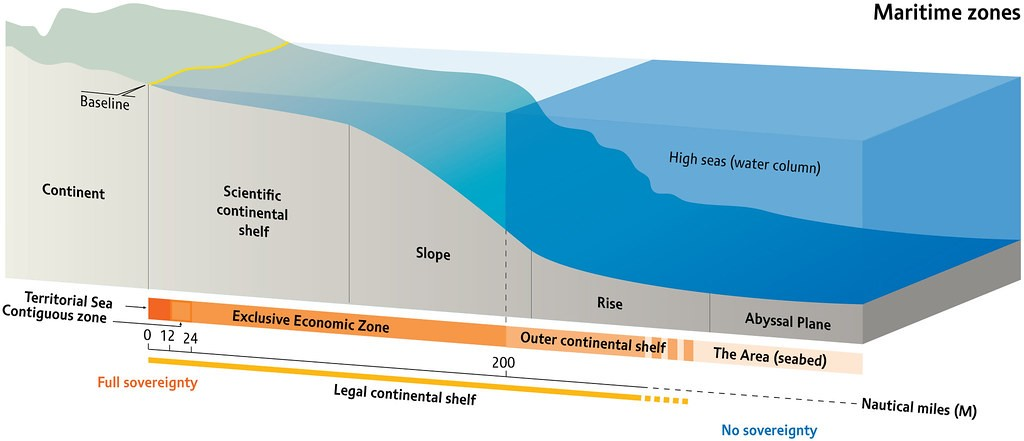
\includegraphics[width=1\textwidth]{Images/UNCLOS Maritime Zones.jpeg}
    \caption{Maritime Zones as Defined in the UNCLOS (Alternative Representation)}
    \label{fig:UNCLOS Maritime Zones}
\end{figure}

\begin{itemize}
    \item There are a number of different lines and zones that are important in international law
    \item Baselines
    \begin{itemize}
        \item Normal baselines follow the contours of the coast in all of its sinuosity, following \convention{\textit{UNCLOS} Art 5} (these are the default baselines)
        \item Straight baselines, which are used in cases primarily where the coast is deeply indented/otherwise irregular, are special baselines that are drawn up upon dots along the coast, following \convention{\textit{UNCLOS} Art 7}
        \item Coastal baselines may take a combination of normal and straight baselines, depending on the complexity and geometry of the coast
        \item Baselines are necessary as a projection point for maritime zones
    \end{itemize}
\end{itemize}

\begin{conventiondetails}{\textit{UNCLOS} Articles 5, 7}
    \flushleft
    \tcbsubtitle{Article 5}
    \textit{Normal baseline}

    \vspace{\baselineskip}

    Except where otherwise provided in this Convention, the normal baseline for measuring the breadth of the territorial sea is the low-water line along the coast as marked on large-scale charts officially recognized by the coastal State.

    \tcbsubtitle{Article 7}
    \textit{Straight baselines}
    \begin{enumerate}
        \item In localities where the coastline is deeply indented and cut into, or if there is a fringe of islands along the coast in its immediate vicinity, the method of straight baselines joining appropriate points may be employed in drawing the baseline from which the breadth of the territorial sea is measured.
        \item Where because of the presence of a delta and other natural conditions the coastline is highly unstable, the appropriate points may be selected along the furthest seaward extent of the low-water line and, notwithstanding subsequent regression of the low-water line, the straight baselines shall remain effective until changed by the coastal State in accordance with this Convention.
        \item The drawing of straight baselines must not depart to any appreciable extent from the general direction of the coast, and the sea areas lying within the lines must be sufficiently closely linked to the land domain to be subject to the regime of internal waters.
        \item Straight baselines shall not be drawn to and from low-tide elevations, unless lighthouses or similar installations which are permanently above sea level have been built on them or except in instances where the drawing of baselines to and from such elevations has received general international recognition.
        \item Where the method of straight baselines is applicable under paragraph 1, account may be taken, in determining particular baselines, of economic interests peculiar to the region concerned, the reality and the importance of which are clearly evidenced by long usage.
        \item The system of straight baselines may not be applied by a State in such a manner as to cut off the territorial sea of another State from the high seas or an exclusive economic zone.
    \end{enumerate}
\end{conventiondetails}

\subsection{Maritime Zones}
\subsubsection{Territorial Sea}
\begin{itemize}
    \item The territorial sea is an inherent, non-claimable zone
    \item It extends 12 nautical miles from the baseline, following \convention{\textit{UNCLOS} Art 3}
    \item States have territorial sovereignty in this area; they own it, and have extensive authority
    \item There are very few exceptions to this authority - the most prevalent is the right of innocent passage
\end{itemize}

\begin{conventiondetails}{\textit{UNCLOS} Articles 2-4}
    \flushleft
    \tcbsubtitle{Article 2}
    \textit{Legal status of the territorial sea, of the air space over the territorial sea and of its bed and subsoil}
    \begin{enumerate}
        \item The sovereignty of a coastal State extends, beyond its land territory and internal waters and, in the case of an archipelagic State, its archipelagic waters, to an adjacent belt of sea, described as the territorial sea.
        \item This sovereignty extends to the air space over the territorial sea as well as to its bed and subsoil.
        \item The sovereignty over the territorial sea is exercised subject to this Convention and to other rules of international law.
    \end{enumerate}

    \tcbsubtitle{Article 3}
    \textit{Breadth of the territorial sea}

    \vspace{\baselineskip}

    Every State has the right to establish the breadth of its territorial sea up to a limit not exceeding 12 nautical miles, measured from baselines determined in accordance with this Convention.

    \tcbsubtitle{Article 4}
    \textit{Outer limit of the territorial sea}

    \vspace{\baselineskip}

    The outer limit of the territorial sea is the line every point of which is at a distance from the nearest point of the baseline equal to the breadth of the territorial sea.
\end{conventiondetails}

\subsubsection{Contiguous Zone}
\begin{itemize}
    \item The contiguous zone is an enforcement zone for customs (the movement of goods), tax, immigration and quarantine laws
    \item It operates in the 12-24 nautical mile range from the baseline, right after the territorial sea, following \convention{\textit{UNCLOS} Art 33(2)}
    \item Coastal states can enforce the law against vessels only in the matters of customs, tax, immigration and quarantine
    \item The origins of this zone go back to the US Prohibition era, when people were attempting to smuggle alcohol into the US
    \item This is not a zone of sovereignty, but is rather a zone of enforcement jurisdiction
\end{itemize}

\begin{conventiondetails}{\textit{UNCLOS} Article 33}
    \flushleft
    \textit{Contiguous Zone}
    \begin{enumerate}
        \item In a zone contiguous to its territorial sea, described as the contiguous zone, the coastal State may exercise the control necessary to:
        \begin{enumerate}[label=(\alph*)]
            \item prevent infringement of its customs, fiscal, immigration or sanitary laws and regulations within its territory or territorial sea;
            \item punish infringement of the above laws and regulations committed within its territory or territorial sea.
        \end{enumerate}
        \item The contiguous zone may not extend beyond 24 nautical miles from the baselines from which the breadth of the territorial sea is measured.        
    \end{enumerate}
    
\end{conventiondetails}

\subsubsection{Exclusive Economic Zone (EEZ)}
\begin{itemize}
    \item This is a creation of \convention{\textit{UNCLOS}}
    \item Coastal states have the right to claim up to 200 nautical miles from the baseline as their exclusive economic zone (per \convention{\textit{UNCLOS} Art 57}), in which they have rights to all of the living and non-living resources (including everything in the soil, subsoil, water column, etc.), and everything on the surface (e.g., renewable energy resources)
    \item This is the most important zone economically
    \item This is not a zone of sovereignty, but is merely a zone where a state has the rights over resources and the right to regulate them
    \begin{itemize}
        \item For example, they cannot forbid foreign ships from passing through, but they can forbid foreign ships from fishing in the zone
    \end{itemize}
\end{itemize}

\begin{conventiondetails}{\textit{UNCLOS} Articles 55-58}
    \flushleft
    \tcbsubtitle{Article 55}
    \textit{Specific legal regime of the exclusive economic zone}

    \vspace{\baselineskip}

    The exclusive economic zone is an area beyond and adjacent to the territorial sea, subject to the specific legal regime established in this Part, under which the rights and jurisdiction of the coastal State and the rights and freedoms of other States are governed by the relevant provisions of this Convention.

    \tcbsubtitle{Article 56}
    \textit{Rights, jurisdiction and duties of the coastal State in the exclusive economic zone}
    \begin{enumerate}
        \item In the exclusive economic zone, the coastal State has:
        \begin{enumerate}[label=(\alph*)]
            \item sovereign rights for the purpose of exploring and exploiting, conserving and managing the natural resources, whether living or non-living, of the waters superjacent to the seabed and of the seabed and its subsoil, and with regard to other activities for the economic exploitation and exploration of the zone, such as the production of energy from the water, currents and winds;
            \item jurisdiction as provided for in the relevant provisions of this Convention with regard to:
            \begin{enumerate}[label=(\roman*)]
                \item the establishment and use of artificial islands, installations and structures;
                \item marine scientific research;
                \item the protection and preservation of the marine environment;
            \end{enumerate}
            \item other rights and duties provided for in this Convention.
        \end{enumerate}
        \item In exercising its rights and performing its duties under this Convention in the exclusive economic zone, the coastal State shall have due regard to the rights and duties of other States and shall act in a manner compatible with the provisions of this Convention.
        \item The rights set out in this article with respect to the seabed and subsoil shall be exercised in accordance with Part VI.
    \end{enumerate}

    \tcbsubtitle{Article 57}
    \textit{Breadth of the exclusive economic zone}

    \vspace{\baselineskip}

    The exclusive economic zone shall not extend beyond 200 nautical miles from the baselines from which the breadth of the territorial sea is measured.

    \tcbsubtitle{Article 58}
    \textit{Rights and duties of other States in the exclusive economic zone}
    \begin{enumerate}
        \item In the exclusive economic zone, all States, whether coastal or land-locked, enjoy, subject to the relevant provisions of this Convention, the freedoms referred to in article 87 of navigation and overflight and of the laying of submarine cables and pipelines, and other internationally lawful uses of the sea related to these freedoms, such as those associated with the operation of ships, aircraft and submarine cables and pipelines, and compatible with the other provisions of this Convention.
        \item Articles 88 to 115 and other pertinent rules of international law apply to the exclusive economic zone in so far as they are not incompatible with this Part.
        \item In exercising their rights and performing their duties under this Convention in the exclusive economic zone, States shall have due regard to the rights and duties of the coastal State and shall comply with the laws and regulations adopted by the coastal State in accordance with the provisions of this Convention and other rules of international law in so far as they are not incompatible with this Part.
    \end{enumerate}
\end{conventiondetails}

\subsubsection{Continental Shelf}
\begin{itemize}
    \item The continental shelf is an inherent seabed resources zone, and a prolongation of a state's territory
    \item States have ownership of the resources on sea bed and the subsoil, and of any living resources that live on the seabed (e.g., crustaceans, sea snails, etc.)
    \item This overlaps to a significant extent with the EEZ
\end{itemize}

\begin{conventiondetails}{\textit{UNCLOS} Articles 76-77}
    \flushleft
    \tcbsubtitle{Article 76}
    \textit{Definition of the continental shelf}

    \begin{enumerate}
        \item The continental shelf of a coastal State comprises the seabed and
        subsoil of the submarine areas that extend beyond its territorial sea
        throughout the natural prolongation of its land territory to the outer edge of
        the continental margin, or to a distance of 200 nautical miles from the
        baselines from which the breadth of the territorial sea is measured where the
        outer edge of the continental margin does not extend up to that distance.
        \item The continental shelf of a coastal State shall not extend beyond the
        limits provided for in paragraphs 4 to 6.
        \item The continental margin comprises the submerged prolongation of the
        land mass of the coastal State, and consists of the seabed and subsoil of the
        shelf, the slope and the rise. It does not include the deep ocean floor with its
        oceanic ridges or the subsoil thereof.
        \item 
        \begin{enumerate}[label=(\alph*)]
            \item For the purposes of this Convention, the coastal State shall establish the outer edge of the continental margin wherever the margin extends beyond 200 nautical miles from the baselines from which the breadth of the territorial sea is measured, by either:
            \begin{enumerate}[label=(\roman*)]
                \item a line delineated in accordance with paragraph 7 by reference to the outermost fixed points at each of which the thickness of sedimentary rocks is at least 1 per cent of the shortest distance from such point to the foot of the continental slope; or
                \item a line delineated in accordance with paragraph 7 by reference to fixed points not more than 60 nautical miles from the foot of the continental slope.
            \end{enumerate}
            \item In the absence of evidence to the contrary, the foot of the
            continental slope shall be determined as the point of maximum
            change in the gradient at its base.
        \end{enumerate}
        \item The fixed points comprising the line of the outer limits of the continental shelf on the seabed, drawn in accordance with paragraph 4 (a)(i) and (ii), either shall not exceed 350 nautical miles from the baselines from which the breadth of the territorial sea is measured or shall not exceed 100 nautical miles from the 2,500 metre isobath, which is a line connecting the depth of 2,500 metres.
        \item Notwithstanding the provisions of paragraph 5, on submarine ridges, the outer limit of the continental shelf shall not exceed 350 nautical miles from the baselines from which the breadth of the territorial sea is measured. This paragraph does not apply to submarine elevations that are natural components of continental margin, such as its plateaux, rises, caps, banks and spurs.
        \item The coastal State shall delineate the outer limits of its continental shelf, where that shelf extends beyond 200 nautical miles from the baselines from which the breadth of the territorial sea is measured, by straight lines not exceeding 60 nautical miles in length, connecting fixed points, defined by coordinates of latitude and longitude.
        \item Information on the limits of the continental shelf beyond 200 nautical miles from the baselines from which the breadth of the territorial sea is measured shall be submitted by the coastal State to the Commission on the Limits of the Continental Shelf set up under Annex II on the basis of equitable geographical representation. The Commission shall make recommendations to coastal States on matters related to the establishment of the outer limits of their continental shelf. The limits of the shelf established by a coastal State on the basis of these recommendations shall be final and binding.
        \item The coastal State shall deposit with the Secretary-General of the United Nations charts and relevant information, including geodetic data, permanently describing the outer limits of its continental shelf. The Secretary-General shall give due publicity thereto.
        \item The provisions of this article are without prejudice to the question of delimitation of the continental shelf between States with opposite or adjacent coasts.
    \end{enumerate}

    \tcbsubtitle{Article 77}
    \textit{Rights of coastal States over continental shelf}

    \begin{enumerate}
        \item The coastal State exercises over the continental shelf sovereign rights for the purpose of exploring it and exploiting its natural resources.
        \item The rights referred to in paragraph 1 are exclusive in the sense that if the coastal State does not explore the continental shelf or exploit its natural resources, no one may undertake these activities without the express consent of the coastal State.
        \item The rights of the coastal State over the continental shelf do not depend on occupation, effective or notional, or on any express proclamation.
        \item The natural resources referred to in this Part consist of the mineral and other non-living resources of the seabed and subsoil together with living organisms belonging to sedentary species, that is to say, organisms which, at the harvestable stage, either are immobile on or under the seabed or are unable to move except in constant physical contact with the seabed or the subsoil.
    \end{enumerate}
\end{conventiondetails}

\subsubsection{High Seas}
\begin{itemize}
    \item These are areas of the sea that are not subject to the jurisdiction of any state, and are open to all states
    \item They cannot be claimed by any state, and are thus non-appropriable
    \item There are certain cardinal freedoms on the high seas that cannot be violated (e.g., navigation, freedom)
\end{itemize}

\begin{conventiondetails}{\textit{UNCLOS} Articles 86-90}
    \flushleft
    \tcbsubtitle{Article 86}
    \textit{Application of the provisions of this Part}

    \vspace{\baselineskip}

    The provisions of this Part apply to all parts of the sea that are not included in the exclusive economic zone, in the territorial sea or in the internal waters of a State, or in the archipelagic waters of an archipelagic State. This article does not entail any abridgement of the freedoms enjoyed by all States in the exclusive economic zone in accordance with article 58.

    \tcbsubtitle{Article 87}
    \textit{Freedom of the high seas}
    \begin{enumerate}
        \item The high seas are open to all States, whether coastal or land-locked. Freedom of the high seas is exercised under the conditions laid down by this Convention and by other rules of international law. It comprises, inter alia, both for coastal and land-locked States:
        \begin{enumerate}[label=(\alph*)]
            \item freedom of navigation;
            \item freedom of overflight;
            \item freedom to lay submarine cables and pipelines, subject to Part VI;
            \item freedom to construct artificial islands and other installations permitted under international law, subject to Part VI;
            \item freedom of fishing, subject to the conditions laid down in section 2;
            \item freedom of scientific research, subject to Parts VI and XIII.
        \end{enumerate}
        \item These freedoms shall be exercised by all States with due regard for the interests of other States in their exercise of the freedom of the high seas, and also with due regard for the rights under this Convention with respect to activities in the Area.
    \end{enumerate}

    \tcbsubtitle{Article 88}
    \textit{Reservation of the high seas for peaceful purposes}

    \vspace{\baselineskip}

    The high seas shall be reserved for peaceful purposes.
    
    \tcbsubtitle{Article 89}
    \textit{Invalidity of claims of sovereignty over the high seas}

    \vspace{\baselineskip}

    No State may validly purport to subject any part of the high seas to its sovereignty.

    \tcbsubtitle{Article 90}
    \textit{Right of navigation}

    \vspace{\baselineskip}
    Every State, whether coastal or land-locked, shall enjoy the right to sail ships flying its fag on the high seas.
\end{conventiondetails}

\subsubsection{Archipelagic Waters}
\begin{itemize}
    \item These were created under \convention{\textit{UNCLOS} Part IV}
    \item These are the waters within an archipelago
    \item All of these waters are held to be very similar to the territorial sea
\end{itemize}

\begin{conventiondetails}{\textit{UNCLOS} Articles 46 - 49}
    \flushleft
    \tcbsubtitle{Article 46}
    \textit{Use of terms}

    \vspace{\baselineskip}

    For the purposes of this Convention:
    \begin{enumerate}[label=(\alph*)]
        \item ``archipelagic State" means a State constituted wholly by one or more archipelagos and may include other islands;
        \item ``archipelago" means a group of islands, including parts of islands, interconnecting waters and other natural features which are so closely interrelated that such islands, waters and other natural features form an intrinsic geographical, economic and political entity, or which historically have been regarded as such.
    \end{enumerate}

    \tcbsubtitle{Article 47}
    \textit{Archipelagic baselines}
    \begin{enumerate}
        \item An archipelagic State may draw straight archipelagic baselines joining the outermost points of the outermost islands and drying reefs of the archipelago provided that within such baselines are included the main islands and an area in which the ratio of the area of the water to the area of the land,including atolls, is between 1 to 1 and 9 to 1.
        \item The length of such baselines shall not exceed 100 nautical miles, except that up to 3 per cent of the total number of baselines enclosing any archipelago may exceed that length, up to a maximum length of 125 nautical miles.
        \item The drawing of such baselines shall not depart to any appreciable extent from the general configuration of the archipelago.
        \item Such baselines shall not be drawn to and from low-tide elevations, unless lighthouses or similar installations which are permanently above sea level have been built on them or where a low-tide elevation is situated wholly or partly at a distance not exceeding the breadth of the territorial sea from the nearest island.
        \item The system of such baselines shall not be applied by an archipelagic State in such a manner as to cut off from the high seas or the exclusive economic zone the territorial sea of another State.
        \item If a part of the archipelagic waters of an archipelagic State lies between two parts of an immediately adjacent neighbouring State, existing rights and all other legitimate interests which the latter State has traditionally exercised in such waters and all rights stipulated by agreement between those States shall continue and be respected.
        \item For the purpose of computing the ratio of water to land under paragraph l, land areas may include waters lying within the fringing reefs of islands and atolls, including that part of a steep-sided oceanic plateau which is enclosed or nearly enclosed by a chain of limestone islands and drying reefs lying on the perimeter of the plateau.
        \item The baselines drawn in accordance with this article shall be shown on charts of a scale or scales adequate for ascertaining their position. Alternatively, lists of geographical coordinates of points, specifying the geodetic datum, may be substituted.
        \item The archipelagic State shall give due publicity to such charts or lists of geographical coordinates and shall deposit a copy of each such chart or list with the Secretary-General of the United Nations.
    \end{enumerate}

    \tcbsubtitle{Article 48}
    \textit{Measurement of the breadth of the territorial sea, the contiguous zone,
    the exclusive economic zone and the continental shelf}

    \vspace{\baselineskip}

    The breadth of the territorial sea, the contiguous zone, the exclusive economic zone and the continental shelf shall be measured from archipelagic baselines drawn in accordance with article 47.

    \tcbsubtitle{Article 49}
    \textit{Legal status of archipelagic waters, of the air space over archipelagic waters and of their bed and subsoil}
    \begin{enumerate}
        \item The sovereignty of an archipelagic State extends to the waters enclosed by the archipelagic baselines drawn in accordance with article 47, described as archipelagic waters, regardless of their depth or distance from the coast.
        \item This sovereignty extends to the air space over the archipelagic waters, as well as to their bed and subsoil, and the resources contained therein.
        \item This sovereignty is exercised subject to this Part.
        \item The regime of archipelagic sea lanes passage established in this Part shall not in other respects affect the status of the archipelagic waters, including the sea lanes, or the exercise by the archipelagic State of its sovereignty over such waters and their air space, bed and subsoil, and the resources contained therein.
    \end{enumerate}

\end{conventiondetails}

\subsubsection{Deep Seabed}
\begin{itemize}
    \item This is referred to as `the Area' in the \convention{\textit{UNCLOS}}, and is considered as the common heritage of mankind
    \item Once an individual/ship leaves the continental shelf and enters the deep seabed, it cannot be appropriated by any state; it is instead vested in all people (i.e., they have a stake in it)
    \item The International Seabed Authority (established by \convention{\textit{UNCLOS}} and based in Jamaica) is responsible for the management of the deep seabed by issuing licences on an equitable basis to ensure all countries can access the resources in the deep sea
    \item The deep sea lies immediately below the high seas
\end{itemize}

\begin{casedetails}{\textit{South China Sea Arbitration (Philippines v China)} [2016] PCA}
    \flushleft
    Prior to 2016, the Philippines challenged China's claim to the entirety of the South China Sea, and to China's assertion of maritime zones from particular features in the Sea. The Tribunal examining these issues was established under \convention{\textit{UNCLOS}}.

    \vspace{\baselineskip}

    The first key issue was China's `Nine-Dash Line', which was held to be incompatible with \convention{\textit{UNCLOS}}. This is because the zone extended very substantially beyond China's coastline, and well beyond the 200 nautical mile limit of the EEZ. The Tribunal held that the Nine-Dash Line was not a valid claim to maritime zones, and that China had no rights to the waters within the line. Moreover, as China was a party to \convention{\textit{UNCLOS}}, any historical claims were extinguished upon the signing of the treaty, and so historical maritime zones could not be argued.

    \vspace{\baselineskip}

    Moreover, none of the maritime features in dispute were islands as defined in \convention{\textit{UNCLOS}}. The Tribunal held that none of the features were capable of generating an EEZ or continental shelf, and that they were all either rocks or low-tide elevations. As such, the Tribunal held that China had no rights to any maritime zones from these features. At most, they could generate a territorial sea, but not an EEZ or continental shelf. The Tribunal also held that China had violated the Philippines' rights in the EEZ, and that China had failed to protect the marine environment in the area.
\end{casedetails}

\section{Antarctica}
\begin{itemize}
    \item There are 7 claimants to territory in Antarctica: Argentina, Australia, Chile, France, New Zealand, Norway, and the UK
    \item Article 4 of the \convention{\textit{1959 Antarctic Treaty}} provides that no new claims to territory in Antarctica may be made, but that there is no renunciation of any existing claims (i.e., they are frozen whilst the treaty is in force)
    \item Whilst the treaty is in force, no acts conducted can constitute a basis for asserting, supporting or denying a claim to territorial sovereignty in Antarctica
\end{itemize}

\begin{conventiondetails}{\textit{1959 Antarctic Treaty} Article 4}
    \flushleft 
    \begin{enumerate}
        \item Nothing contained in the present Treaty shall be interpreted as:
        \begin{enumerate}[label=(\alph*)]
            \item a renunciation by any Contracting Party of previously asserted rights of or claims to territorial sovereignty in Antarctica;
            \item a renunciation or diminution by any Contracting Party of any basis of claim to territorial sovereignty in Antarctica which it may have whether as a result of its activities or those of its nationals in Antarctica, or otherwise;
            \item prejudicing the position of any Contracting Party as regards its recognition or non-recognition of any other State's right of or claim or basis of claim to territorial sovereignty in Antarctica.
        \end{enumerate}
        \item No acts or activities taking place while the present Treaty is in force shall 
        constitute a basis for asserting, supporting or denying a claim to territorial 
        sovereignty in Antarctica or create any rights of sovereignty in Antarctica. No new 
        claim, or enlargement of an existing claim, to territorial sovereignty in Antarctica 
        shall be asserted while the present Treaty is in force.
    \end{enumerate}
\end{conventiondetails}

\section{Airspace and Outer Space}

\subsection{Airspace}
\begin{itemize}
    \item A state has sovereignty over the airspace above its territory and territorial sea (\textit{cujus est solum ejus est usque ad coelum})
    \item Other states have the freedom of overflight over the contiguous zone, the EEZ, and high seas
    \item The boundary between national airspace and outer space is not clearly defined
\end{itemize}

\subsection{Outer Space}
\begin{itemize}
    \item The \convention{\textit{1967 Outer Space Treaty} Art 2} provides that outer space is not subject to national appropriation by any means
    \item Article 1 of this treaty additionally holds that outer space is the province of mankind
    \item There are 113 parties to this treaty
\end{itemize}

\begin{conventiondetails}{\textit{1967 Outer Space Treaty}}
    \flushleft
    \tcbsubtitle{Article 1}
    The exploration and use of outer space, including the moon and other celestial bodies, shall be carried out for the benefit and in the interests of all countries, irrespective of their degree of economic or scientific development, and shall be the province of all mankind.

    \vspace{\baselineskip}
    
    Outer space, including the moon and other celestial bodies, shall be free for exploration and use by all States without discrimination of any kind, on a basis of equality and in accordance with international law, and there shall be free access to all areas of celestial bodies.

    \vspace{\baselineskip}
    
    There shall be freedom of scientific investigation in outer space, including the moon and other celestial bodies, and States shall facilitate and encourage international co-operation in such investigation.
    \tcbsubtitle{Article 2}
    Outer space, including the moon and other celestial bodies, is not subject to national appropriation by claim of sovereignty, by means of use or occupation, or by any other means.
\end{conventiondetails}

\begin{itemize}
    \item The \convention{\textit{1979 Moon Agreement} Art 11(1)} provides that the moon and other celestial bodies are the common heritage of mankind
    \item There are only 18 parties to this treaty
\end{itemize}

\begin{conventiondetails}{\textit{1979 Agreement Governing the Activities of States on the Moon and Other Celestial Bodies} Article 11}
    \flushleft
    \begin{enumerate}
        \item The moon and its natural resources are the common heritage of mankind, which finds its expression in the provisions of this Agreement, in particular in paragraph 5 of this article.
        \item The moon is not subject to national appropriation by any claim of sovereignty, by means of use or occupation, or by any other means.
        \item Neither the surface nor the subsurface of the moon, nor any part thereof or natural resources in place, shall become property of any State, international intergovernmental or non- governmental organization, national organization or non-governmental entity or of any natural person. The placement of personnel, space vehicles, equipment, facilities, stations and installations on or below the surface of the moon, including structures connected with its surface or subsurface, shall not create a right of ownership over the surface or the subsurface of the moon or any areas thereof. The foregoing provisions are without prejudice to the international regime referred to in paragraph 5 of this article.
        \item States Parties have the right to exploration and use of the moon without discrimination of any kind, on the basis of equality and in accordance with international law and the terms of this Agreement.
        \item States Parties to this Agreement hereby undertake to establish an international regime, including appropriate procedures, to govern the exploitation of the natural resources of the moon as such exploitation is about to become feasible. This provision shall be implemented in accordance with article 18 of this Agreement.
        \item In order to facilitate the establishment of the international regime referred to in paragraph 5 of this article, States Parties shall inform the Secretary-General of the United Nations as well as the public and the international scientific community, to the greatest extent feasible and practicable, of any natural resources they may discover on the moon.
        \item The main purposes of the international regime to be established shall include:
        \begin{enumerate}[label=(\alph*)]
            \item The orderly and safe development of the natural resources of the moon;
            \item The rational management of those resources;
            \item The expansion of opportunities in the use of those resources;
            \item An equitable sharing by all States Parties in the benefits derived from those resources, whereby the interests and needs of the developing countries, as well as the efforts of those countries which have contributed either directly or indirectly to the exploration of the moon, shall be given special consideration.
        \end{enumerate}
        \item All the activities with respect to the natural resources of the moon shall be carried out in a manner compatible with the purposes specified in paragraph 7 of this article and the provisions of article 6, paragraph 2, of this Agreement.
    \end{enumerate}
\end{conventiondetails}